\beginsong{Dort an dem Üferchen}[
    txt={utta (Gustav Kemperdick)}, 
    mel={russische Volksweise}, 
    bo={86}, 
    pfii={41}, 
    pfiii={19}, 
    gruen={14}, 
    siru={58}, 
    index={Kasanka},
]

\beginverse
\endverse
\centering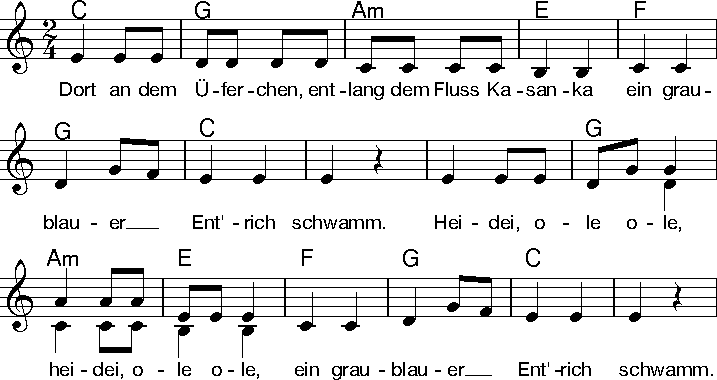
\includegraphics[width=1\textwidth]{Noten/Lied029.pdf}	

\beginverse
\[C]Dort an dem \[G]Üferchen ent\[Am]lang dem Fluss Ka\[E]sanka \[F]ein gar \[G]guter \[C]Bursche ging.
Heidei, o\[G]le ole, \[Am]heidei, o\[E]le ole, \[F]ein gar \[G]guter \[C]Bursche ging.
\endverse

\beginverse
^Sieh, da kommt ein ^Reiter, ^führt ein ledig ^Pferd; der ^Bursch' be^hend hi^nauf sich schwingt.
Heidei, o^le ole, ^heidei, o^le ole, der ^Bursch' be^hend hi^nauf sich schwingt.
\endverse

\beginverse
^Bursch', willst du nicht ^bleiben ^bei der lieben ^Mutter ^und dem ^greisen ^Vater dein? 
Heidei, o^le ole, ^heidei, o^le ole, ^und dem ^greisen ^Vater dein?
\endverse

\beginverse
^Sieh, ich lieb' die ^Mutter ^und den greisen ^Vater, ^doch die bunten ^Mützen der Ko^saken lieb ich mehr.
Heidei, o^le ole, ^heidei, o^le ole, ^doch die bunten ^Mützen der Ko^saken lieb ich mehr.
\endverse

\beginverse
^Dort auf der ^Brücke ^steht ein junges ^Mädchen, ^Tränen ^tropfen ^in den Fluss.
Heidei, o^le ole, ^heidei, o^le ole, ^Tränen ^tropfen ^in den Fluss.
\endverse

\beginverse
^Dort an dem ^Üferchen, ent^lang dem Fluss Ka^sanka, ^reiten zwei ^junge Ko^saken dahin. 
\lrep Heidei, o^le ole, ^heidei, o^le ole, ^reiten zwei ^junge Ko^saken dahin. \rrep
\endverse


\endsong

\beginscripture{}
Die Kasanka ist ein Nebenfluss der Wolga in der Republik Tatarstan im europäischen Teil Russlands. ''Kosaken'' (bedeutet in etwa ''freie Krieger'') waren Gemeinschaften freier Reiterverbände aus flüchtigen russischen und ukrainischen Leibeigenen.
\endscripture
